\begin{exercício}{Placas paralelas parcialmente preenchidas com material dielétrico}{exercício4}
    Considere duas placas metálicas quadradas de lado \(L\) e espessuras desprezíveis. As placas estão paralelas e separadas por uma distância \(d\). Assuma que os planos das placas são paralelos ao plano \(xy\), que a placa inferior (superior) está em \(z = 0\) (\(z = d\)) e que estão orientadas como mostra a figura abaixo.

    \begin{center}
        \begin{tikzpicture}[scale=0.8, every node/.style={scale=0.8}]
            \draw[-stealth] (-3.,0,0) -- (3.,0,0) node[below] {$y$};
            \draw[-stealth] (0,-.5,0) -- (0,2.5,0) node[left] {$z$};
            \draw[-stealth] (0,0,-2.5) -- (0,0,2.5) node[below right] {$x$};

            \draw[fill=Overlay0, opacity=0.7] (-2.5,0,-1.5) -- (2.5,0,-1.5) -- (2.5,0,1.5) -- (-2.5,0,1.5) -- cycle;
            \draw (2.5,0,-1.5) node[right] {$\phi = 0$};

            \draw[fill=Overlay0, opacity=0.7] (-2.5,1.5,-1.5) -- (2.5,1.5,-1.5) -- (2.5,1.5,1.5) -- (-2.5,1.5,1.5) -- cycle;
            \draw (2.5,1.5,-1.5) node[right] {$\phi = \phi_0$};

            \draw[stealth-stealth] (-2.5,0,1.5) -- (-2.5,1.5,1.5) node[midway, anchor=east] {\(d\)};
        \end{tikzpicture}
    \end{center}
    A placa superior está mantida a um potencial \(\phi_0>0\), enquanto que a placa inferior está aterrada. Assumamos que \(d \ll L\), de forma que podemos desprezar quaisquer efeitos de borda. Adicionalmente, um dielétrico de constante dielétrica \(k\) preenche \emph{metade} da região entre as placas, e duas configurações serão consideradas, como mostram as figuras abaixo, onde \(\epsilon = k \epsilon_0\).

    \begin{center}
        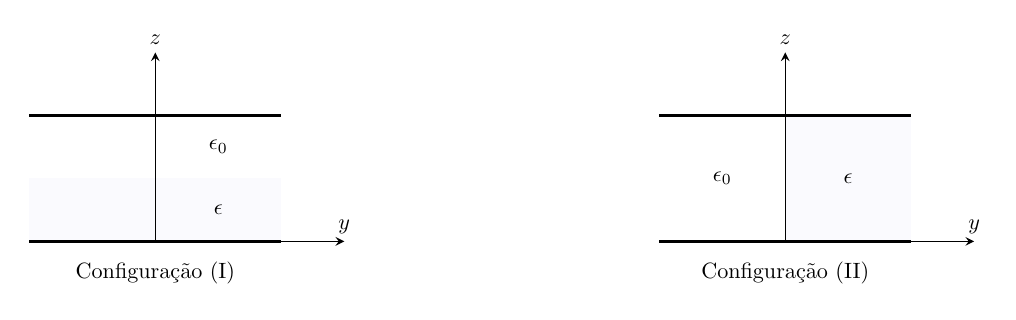
\begin{tikzpicture}[scale=0.8, every node/.style={scale=0.8}]
            \fill[Lavender!20] (0,0) rectangle (4,1);
            \draw[very thick] (0,2) -- (4,2);
            \draw[very thick] (0,0) -- (4,0);

            \node at (3,1.5) {$\epsilon_0$};
            \node at (3,0.5) {$\epsilon$};

            \draw[-stealth] (2,0) -- (2,3) node[above] {$z$};
            \draw[-stealth] (0,0) -- (5,0) node[above] {$y$};

            \node at (2,-0.5) {Configuração (I)};
            \begin{scope}[xshift=10cm]
                \fill[Lavender!20] (2,0) rectangle (4,2);
                \draw[very thick] (0,2) -- (4,2);
                \draw[very thick] (0,0) -- (4,0);

                \node at (1,1) {$\epsilon_0$};
                \node at (3,1) {$\epsilon$};

                \draw[-stealth] (2,0) -- (2,3) node[above] {$z$};
                \draw[-stealth] (0,0) -- (5,0) node[above] {$y$};

                \node at (2,-0.5) {Configuração (II)};
            \end{scope}
        \end{tikzpicture}
    \end{center}

    Calcule a energia eletrostática armazenada em toda a região entre as placas em cada configuração. Dado que \(k > 1\), em qual das duas configurações a energia é maior?
\end{exercício}
\begin{proof}[Resolução]

\end{proof}
